\documentclass{article}
\usepackage[utf8]{inputenc}
\usepackage[russian]{babel}
\usepackage{graphics}
\usepackage{amsfonts}
\usepackage{amssymb}

\ifx\pdfoutput\undefined
\usepackage{graphicx}
\else
\usepackage[pdftex]{graphicx}
\fi

\hoffset -2.0cm	
\voffset -3.0cm
\textheight 23.5cm 
\textwidth 17.0cm

\title{\bf Отчет \No 3}
\author{Амосов Федор}

\begin{document}
	\maketitle
	
	\begin{center}
	    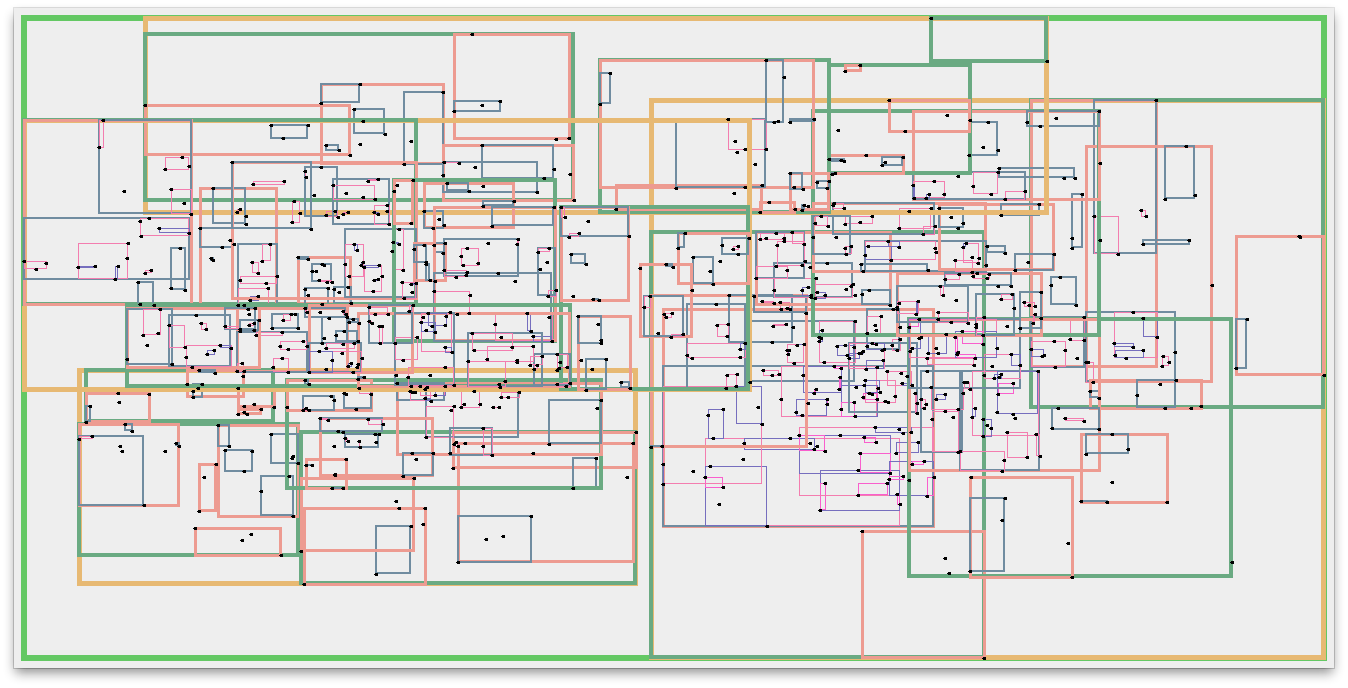
\includegraphics[scale = 0.25]{r-tree.png}
	\end{center}
	
	
    После реализованного построения R--Tree, можно с уверенностью добавить базу в псевдокоде алгорима,
	
	\paragraph{Алгоритм \\}
	    Дано множество $d$ мерных точек $P = \{p_i\}_{i = 1}^n$. Требуется реализовать построение VoRTree на этих точках с помощью MapReduce.
	   

        {\tt
            \phantom ~~ \\
            \phantom ~$u_{min}$, $u_{max}$ = min and max number of sons    \\
            \phantom ~$f$ = some 2--dimension function    \\
            \phantom ~$m$ = number of java vitual machines in cluster    \\
            
            \noindent M-Tree(Points $P$) \{ \\
            \phantom ~~~~$root$ = new Node    \\
            \phantom ~~~~radius of $root$ = min radius of ball, which contains $P$    \\
            \phantom ~~~~$k$ = $f$($u_{min}$, $u_{max}$)    \\
            \phantom ~~~~if (|$P$| < $k$) \{    \\
            \phantom ~~~~~~~~add $P$ to $root$    \\
            \phantom ~~~~~~~~$T$ = new Tree only with $root$    \\
            \phantom ~~~~~~~~return $T$    \\
            \phantom ~~~~\}    \\            
            \phantom ~~~~$S$ = get $k$ different random points from $P$      \\
            \phantom ~~~~\{$P_i$\} = split $P$ into $m$ parts    \\
            \phantom ~~~~\{Pair<$s_i$, $P_{s_i}$>\} = MapReduce(\{Pair<$P_i$, $S$>\})    \\  
            \phantom ~~~~for $P_{s_i}$ in \{$P_{s_i}$\} \{   \\ 
            \phantom ~~~~~~~~$T_{s_i}$ = M-Tree($P_{s_i}$)    \\
            \phantom ~~~~\}    \\
            \phantom ~~~~$T$ = hang \{$T_{s_i}$\} by $root$    \\
            \phantom ~~~~return $T$    \\ 
                     \}    \\
            
            \noindent map(Pair<Points $P$, Points $S$>) \{    \\
            \phantom ~~~~for $p$ in $P$ \{    \\
            \phantom ~~~~~~~~$s$ = closest to $p$ from $S$    \\
            \phantom ~~~~~~~~to output: map.entry(s, p)    \\  
            \phantom ~~~~\}    \\   
                     \}    \\
                     
            \noindent reduce(Point $s$, Points $P_s$) \{    \\
            \phantom ~~~~return map.entry($s$, $P_s$)    \\         
                     \}
        }
        
    \paragraph{Вопросы}
        \begin{enumerate}
            \item На самом деле, интересно следующее. После того, как в строчке {\tt \{Pair<$s_i$, $P_{s_i}$>\} = MapReduce(\{Pair<$P_i$, $S$>\}) } отработает MapReduce, все JVM кластера бездействуют. На самом деле, далее они будут загружены внутри рекурсивного построения, но все же, было бы интересно каждое $T_{s_i}$ строить на отдельной JVM. Ясно, что тогда будет рекурсия в MapReduce, что не совсем понятно. Поэтому, хотелось бы узнать что-нибудь о схеме кластера машин и об общении JVM внутри кластера.
            \item Когда лучше делать запрос к базе данных? Если в Mapper, то получится слишком много запросов, если перед MapReduce, то надо будет хранить слишком много точек в оперативной памяти.
            \item Честно говоря, я не нашел готовой симплексикации Делоне в $d$--мерном пространстве. Есть только для плоскости. Неужели ее придется писать самому?
            \item Как искать объемлющую сферу в евклидовой метрике? Это сложная задача --- именно поэтому мы используем объемлющие прямоугольники?
            \item Откуда точки будут появляться в базе данных? Они там изначально будут, или мы их туда засунем из файла? 
            \item Есть еще несколько технических вопросов. Но я их пока что не могу сформулировать, ввиду того, что я еще не закоммитил соответствующий код.
             
        \end{enumerate}
	
	
	
	
\end{document}